\chapter{Personnes, familles et âges}\label{ch:personnes}

\section{Compter des personnes, non des notices}

La première version du catalogue relevait un seul âge par notice : pour un texte qui commémore plusieurs défunts, seul le premier était retenu. La base de travail contient désormais une table des personnes, où chaque mention d’âge forme une ligne distincte des durées de mariage. Cette table a été contrôlée sur le texte transmis pour la présente édition. Le contrôle a conduit à dix corrections :

\begin{itemize}
\item au \nnum{411}, l’âge est \emph{annorum viginti duo}, vingt-deux ans, et non vingt ;
\item au \nnum{400}, les « 17 jours » de la table provenaient de la date (\emph{VIIIIX K(a)l(endas) Mart(ias)}) ;
\item au \nnum{133}, la première « personne » (3 ans et 10 mois) est la durée de la vie commune d’Agrippina et de Felix (\emph{cum quo vixit sine laesione animi annos III et m(enses) X}) ;
\item au \nnum{19}, la seconde « personne » (22 jours) est la durée du séjour de Santulus à Rome (\emph{Romae vixit d(ies) XXII}) ;
\item au \nnum{364}, l’âge de cinq ans de la table est la durée restituée du mariage ; seules les unités de l’âge sont conservées (\emph{[- - -]ta et quinque}) ;
\item aux \nnums{53}, 83, 184, 324 et 365, les mois et les jours attribués à l’âge appartiennent à la durée du mariage ou à la date.
\end{itemize}

Après correction, l’ensemble C compte \st{nPersAge} personnes dont l’âge est indiqué. Pour \st{nAgeAns} d’entre elles, l’âge comporte un nombre d’années ; il est entièrement lu pour \st{nAgeAnsLu}. Pour les \st{nAgeMoisJours} autres, seuls des mois ou des jours sont conservés. Dans la plupart de ces cas, le nombre d’années est perdu dans une lacune ; un seul texte donne avec certitude l’âge d’un enfant mort avant un an (Aristo, \emph{puer innox}, huit mois, \nnum{308}). Six textes indiquent l’âge de plusieurs personnes : \nnums{\st{multiageslist}}.

\section{Les âges déclarés}

L’âge médian des \st{nAgeAns} personnes dont l’âge est exprimé en années est de \st{ageMed} ans, et l’âge moyen de \st{ageMoy} ans ; pour les seuls âges entièrement lus, ces valeurs sont de \st{ageMedLu} et \st{ageMoyLu} ans. La répartition par décennies (figure~\ref{fig:ages}) montre une forte représentation des enfants : 43 personnes ont moins de dix ans, soit près d’un quart des âges exprimés en années.

\begin{figure}[tbp]\centering
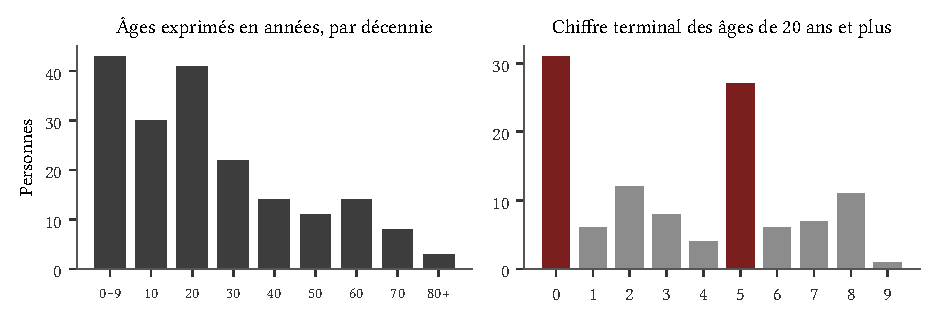
\includegraphics[width=\linewidth]{figures/fig_ages.pdf}
\caption{À gauche : âges exprimés en années, par décennie (ensemble C, n = \st{nAgeAns}). À droite : chiffre terminal des âges de vingt ans et plus (n = \st{nAges20}) ; en rouge, 0 et 5.}\label{fig:ages}
\end{figure}

Ces nombres ne mesurent pas la mortalité. La commémoration épigraphique sélectionne les défunts selon l’âge, le sexe, le statut et la famille ; les enfants y sont surreprésentés par rapport aux adultes âgés, et la part des jeunes enfants commémorés ne peut être assimilée à leur poids démographique. Les travaux de Hopkins, de Shaw et de Scheidel (chapitre~\ref{ch:historiographie}) interdisent de tirer de ces chiffres une espérance de vie.

\section{L’arrondi des âges}

L’attraction des âges ronds est très marquée. Sur les \st{nAges20} âges de vingt ans et plus, 31 se terminent par 0 et 27 par 5 : plus de la moitié, alors qu’une déclaration exacte en donnerait environ un cinquième. Pour les âges de 23 à 62 ans, l’indice de Whipple atteint \st{whipple} (\st{whippleN} personnes) et \st{whippleLu} pour les seuls âges entièrement lus (\st{whippleLuN} personnes) ; la valeur 100 correspond à l’absence d’attraction, 500 à une déclaration exclusivement en multiples de cinq. L’expression \emph{plus minus}, présente pour \st{nPlusMinus} personnes, va dans le même sens : pour une part notable des adultes, l’âge gravé est une estimation, et le texte le dit.

À l’inverse, la précision au mois et au jour se rencontre surtout pour les enfants. Un seul texte donne une durée en heures sans restitution : Ianuaria a vécu 24 ans, un jour et deux heures et demie (\emph{annos XXIIII diem I horas II s(emis)}, \nnum{118}). Aux \nnums{287} et 305, la mention des heures est restituée.

\section{La vie conjugale}

Vingt-trois textes indiquent la durée de la vie commune, souvent avec la même précision que l’âge (\emph{fecit cum marito annos…}, \emph{vixit mecum…}, \emph{in coniugio fecit…} ; tableau~\ref{tab:conjugale}). Lorsque l’âge et la durée du mariage sont tous deux conservés, ils permettent d’estimer l’âge au mariage. Sabina, morte à quinze ans, a été mariée deux ans (\nnum{200}) ; Paternia, morte « à environ quarante ans », vingt ans (\nnum{223}) ; Caelestina, morte à vingt ans, quatre ans (\nnum{399}). Le \nnum{324} distingue en outre les fiançailles : Hilaritas, fiancée à onze ans, le reste sept ans, puis vit sept ans et huit mois avec son mari ; le mariage a donc eu lieu vers dix-huit ans, et la somme (25 ans et 8 mois) concorde avec l’âge gravé, \emph{ann(os) XXV}.

% généré par scripts/04_generated.py
\begin{longtable}{@{}r r p{0.75\linewidth}@{}}\caption{Durées de vie commune déclarées (ensemble C ; extrait du texte transmis).}\label{tab:conjugale}\\\toprule N° & Année & Passage\\\midrule\endfirsthead\bottomrule\endfoot
4 & 341 & \lat{⸢v⸣ixit / cum ⸢v⸣(i)rg(i)nia annis XV bene merenti ⸢v⸣irginia sua Bictora /} \\
21 & 347 & \lat{fecit cum m[arito annos / quae vixit a]nn(os) XXXV m(enses) II d(ies)} \\
26 & 348 & \lat{vixit mecum / annos XVIII m(enses) V d(ies) XXV Aradius} \\
40 & 353 & \lat{⸢v⸣ix⸢i⸣t cum co/[niuge sua annos] XXI me(n)s(es) III depositus / [annoru]} \\
53 & 358 & \lat{vixit cum marito / [annos] m(enses) VIII} \\
83 & 364 & \lat{fecit [mecum] / m(enses) VI d(ies) XXII dep(osita) in p(ace)} \\
135 & 369 & \lat{fecit mecum a(n)n(os) XV / [Va]lentiniano ⸢d⸣(omino) n(ostro)} \\
184 & 375 & \lat{fecit cum co⸢m⸣pare suo m(enses) X d(ies) V / Kal(endis) No⸢v⸣(embribus)} \\
185 & 375 & \lat{fecit mecum annos XX} \\
193 & 376 & \lat{fecit cum marito ann⸢o⸣s plus minus quin/decim et dies duodecim} \\
200 & 377 & \lat{in coniu(gio) fec(it) ann(os) II} \\
219 & 381 & \lat{vixit cu[m marito suo] / IIII ⸢F⸣l(avio) Sy[agrio]} \\
223 & 381 & \lat{fecit cu/m marito suo an(nos) XX / discessit pri(die) Kal(endas) /} \\
254 & 383 & \lat{[fecit c]um marit[o annos] / Merob[aude II et Saturnino conssulibu]} \\
265 & 384 & \lat{fecit cum virginio suo an[nos / Rico]mere et Clearcho consulib} \\
286 & 386 & \lat{fecit cum vi[rginia sua annos consu]/latu Honori[o nobilissimo pu]} \\
291 & 387 & \lat{[fecit cum ma]rit⸢o⸣ ann[os] dies X [recessit / in pace K]al(endas) Ia} \\
324 & 390 & \lat{vixit cum marito ann(os) VII menses VIII deposita die XVII Kal(en)} \\
364 & 394 & \lat{fec⸢i⸣t / [cum coniuge s]ua Donata dulcissima / [annos quinqu]e depos} \\
365 & 394 & \lat{fecit / cum co⸢m⸣pare sua ann⸢o⸣s septe(m) / mens⸢e⸣s VIIII bene merent} \\
373 & 395 & \lat{fecit cum [marito suo annos] / dies III deposita / conss(ulib)} \\
399 & 397 & \lat{fecit cum marito annos V d(ies) VI / deposita IIII Non(as) Iul(ias)} \\
420 & 398 & \lat{fecit cu[m coniuge suo] / d(ies) LXX in p(ace)} \\
\end{longtable}


L’emploi de \emph{virginius} et de \emph{virginia} pour désigner l’époux ou l’épouse épousé vierge est attesté sans restitution dans trois textes (\nnums{4}, 218 et 265) et restitué dans deux autres (\nnums{45} et 286). Au \nnum{4}, Iunianus a vécu quinze ans « avec sa \emph{virginia} » Victora (\emph{Bictora}), qui fait graver l’épitaphe ; les deux époux sont qualifiés d’\emph{amator} et d’\emph{amatrix pauperum}. Ce vocabulaire appartient aux épitaphes chrétiennes de Rome ; il valorise le mariage unique, sans permettre d’en mesurer la fréquence.

\section{Les enfants}

Les épitaphes d’enfants ont un vocabulaire propre. \emph{Innocens}, \emph{innox} et \emph{dulcissimus} qualifient l’enfant ; \emph{puer} et \emph{puella} sont employés jusqu’à l’adolescence (Ursa, \emph{puella} de vingt-deux ans, au \nnum{411} ; Sabina, \emph{puella} mariée, au \nnum{200}). Deux enfants sont dits \emph{neofytus} : Aristo, mort à huit mois (\nnum{308}), et Quiminatus, mort à environ cinq ans (\nnum{210}). Ces deux textes attestent le baptême d’enfants jeunes, peut-être administré à l’approche de la mort ; ils sont repris au chapitre~\ref{ch:foi_eglise}.
